\documentclass[american]{scrartcl}

    \newcommand{\lang}{en}

    \usepackage{babel}
    \usepackage[utf8]{inputenc} 
    \usepackage{csquotes}
    \usepackage{amsmath}
    \usepackage{graphicx}    

    \setlength{\parindent}{0em}
    \setlength{\parskip}{0.5em}


    \usepackage[
        bibencoding=utf8, 
        style=apa
    ]{biblatex}

    \bibliography{refs}
    
    
    \usepackage{amsmath}
    \title{
        Trophic Analysis of a Prosumer Electricity Market
    }

    \author{Andrea Titton}
    
\begin{document}

% \nocite{*}
\maketitle

\section{Introduction}



The ongoing energy market transition, from centralized and oligopolistic fossil fuel producers to distributed renewable energy prosumers, calls for a shift in economic modelling, both in methodology and objectives. A shift is needed in methodology because the network structure and heterogeneity of producers add fundamental non-linearities in the market clearing mechanism. With regards to objectives, questions of efficiency and resilience in complex networks cannot be addressed through a traditional homogenous policy, but require understanding of the heterogenous dynamics within the market structure.

\section{Research Question}

The project's main objective will be to identify the conditions under which a decentralized prosumer market for electricity displays aggregate resilience.

The research question will be dealt with on three dependent levels. First, the resilience properties will be investigated within a theoretical framework. Second, based on the theoretical model, an empirical analysis will be formulated. Third, the empirical result will define suitable policy implications.

\section{Methodology}

\subsection{Notion of resilience}

The notion of network resilience will be mapped to three properties of dynamical systems: systemic stability, self-organized critical dynamics, and Lyapunov stability.

The first arises when a network's critical points are robust to perturbations of its nodes. For example, a desirable property for an electricity market of prosumers is its ability to prevent systematic shortages following a climate shock. The second, as presented by \citeauthor{Bak1995} (\citeyear{Bak1995}), concerns the ability of the system to evolve towards critical points with the same characteristics, regardless of the parameters and scale. In the context of our model, this implies that the pricing mechanism and equilibria of the proposed market should display scale-invariant characteristics. The third property refers to the stability of a solution near the equilibrium. Applied to a prosumer electricity market, it is desirable for the equilibrium price vector of electricity to be stable around the market clearing price. %FIXME: Remove the list structure

\subsection{Theoretical model}

The electricity market will be modeled as an exogenous cyclical network, where each node is a prosumer and each edge represents the possibility of trading electricity between two nodes (or of storing electricity at a cost, if the edge's source is the same as its target). The exogenous network will be based on \citeauthor{Brown2019} (\citeyear{Brown2019}).

Prosumers are assumed to be heterogenous, risk-averse agents with bounded rationality, making decisions in discrete time. Heterogeneity will be modeled over two dimensions: agents have different degrees of risk tolerance and use different price forecasting rules. The former yields a model that allows for a price system where less risk-averse users bear more risk and absorb the shock uncertainty for other users. The latter allows for the model to display spatial herd behavior, that is prosumers behaving similarly within network clusters. % FIXME: Remove the list structure

The agents' behavior will be driven by a dynamic optimization problem in discrete time. In particular, agents maximize profit given current price, expected price dynamics, and an inelastic demand of energy. The two heterogeneities can be incorporated in this framework by using Epstein-Zin preferences in the formulation of the Bellman equation.

Furthermore, two pricing mechanisms will be considered on the market. First, a centralized energy price, either generated exogenously by the government under complete information or endogenously via an auction mechanism. Second, a vector of prices (one for each edge) that solves the bargaining problems between two nodes, derived as in \citeauthor{Bedayo2016} (\citeyear{Bedayo2016}). % FIXME: No verb

Given the structure of the model, the goal is to derive a law of motion (i.e. non-linear difference equation) for electricity production and analyze its dynamical properties. In particular the focus will be on finding the combination of parameter space, pricing mechanism, and network structure that yields the optimal resilience, as defined above.

\iffalse
    \begin{figure}[h!]
        \centering
        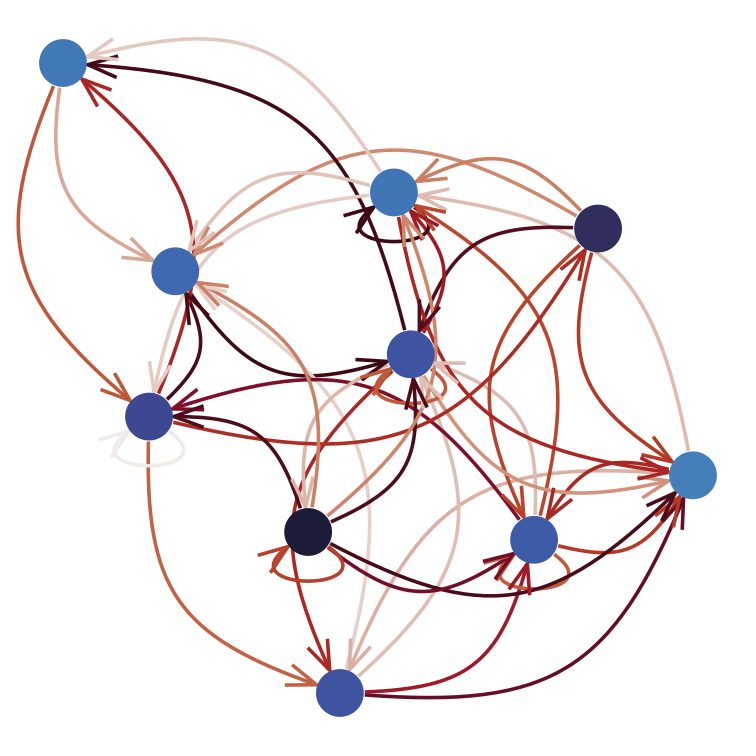
\includegraphics[width=\linewidth,height=0.4\textheight,keepaspectratio]{../../plots/presentations/electricity.png}
        \label{fig:random_example}
        \caption{A potential realization of the described model}
    \end{figure}
\fi

\subsection{Trophic Analysis}

To simplify the problem space and ease the empirical testability of the model, we will use techniques from trophic analysis.

The goal is to create a link between the model's structure and its dynamics, analogous to \citeauthor{MacKay2020} (\citeyear[p.~19]{MacKay2020}), by deriving a formula for the trophic levels and associated trophic incoherence value ($F_0$), defining a set of shocks the network could face, and then expressing the resilience to such shocks as a function of $F_0$.

Using trophic coherence as a pivot to the model's dynamics, as opposed to more traditional economic metrics such as upstreamness (\cite{Antrs2012}), offers three main advantages. First, it does not require ``source'' nodes in directed graphs, hence it is defined for cycle graphs. Second, it is robust to local computation, that is, assuming we can only observe or model a subgraph, the trophic levels are constant in the inner graph and do not vary drastically around truncations (\cite[p.~19]{MacKay2020}). Third, its interpretation is fundamentally linked to that of the \textit{spectral radius} of a graph, which regulates the behavior of most dynamical systems on graphs, despite being simpler to measure.

These three properties allow for an empirically and theoretically consistent, robust, and easily computable metric that acts as a window on the inner workings of the network's dynamics.


\subsection{Empirical testability}

The calibration and empirical analysis needs to estimate both agent specific characteristics, namely attitude towards risk and forecasting rule, as well as structural network characteristics, namely the number of prosumers and their respective possibility to trade. The network structural characteristics can be estimated using existing datasets such as the \textit{Open Power System Data} (\cite{Wiese2019}). Given the networks structure, one can estimate the former using survey data on price expectations.

% TODO: Add more on empirical strategy

\subsection{Policy implications}

The last step of the analysis will consist of testing various potential policies on the developed model. Of particular interest are dynamic policies, such as taxation or subsidies, and structural policies, such as constructing new edges (i.e. cables between prosumers or batteries), which allow the system to converge to a more resilient system via the least disruptive path.

% TODO: Expand on the policy

\newpage
\pagenumbering{gobble} % stop page numbering

\printbibliography
\end{document}